\section{Actor basierte Architekturmuster}\label{sec:theory:actorArchitecture}
Die Entwicklung von gängigen Designmustern wie beispielsweise jene der \textit{Game of Four} (siehe \cite{gangOfFour1995design}), sind auf die Objektorientierte Programmierung ausgerichtet. Im \textit{Actor Model} können eine vielzahl dieser Muster nicht mehr verwendet werden bzw. ihre stärken nicht mehr optimal ausspielen. Um die stärken des \textit{Actor Models} optimal auszuspielen sind etliche Architekturmuster entstanden, welche unter anderem in \cite{Vernon2015ReactiveAkka} und \cite{kuhn2017reactive} beschrieben werden. Einige dieser Muster werden nachfolgend beschrieben um die Verständlichkeit mit der Arbeit des \textit{Actor Models} zu erhöhen.

\subsection{Request-Replay}
Das einfachste, und gleichzeitig wohl wichtigste Muster innerhalb des \textit{Atore-Models} ist das \textit{Request-Replay} Muster. Es wird benötigt Inhalte von einem Actor abzufragen. Wie in \ref{actor:requirements:shareNothing} beschrieben, darf ein Actor keine Informationen nach außen geben. Möchte nun ein Actor Informationen von einem anderen Actor haben, so muss dieser eine Nachricht an den betroffenden Actor senden, dieser sendet dann eine neue Nachricht, mit den entsprechenden Informationen, an den anfragenden Actor zurück. Die Antwort Nachricht kommt dabei nicht als direkte Antwort der Nachricht, sondern als eigenständige Nachricht an den fragenden Actor zurück. Es wird zwar von der Antwort gesprochen, wie jedoch in \ref{actor:requirements:AsynchronCommunication} beschrieben ist jede Anfrage an einen Actor asynchron. Deshalb wird die Antwort wieder in die Mailbox des Empfängers zugesendet. Zur vereinfachung wird jedoch von einer Antwort Nachricht gesprochen. \\
In der Abbildung \ref{fig:actor:patterns:requestReplay} ist das \textit{Request-Replay} abgebildet. Der Actor \textit{A} sendet eine \textit{Command-Message} an den Actor \textit{B}, dieser Verarbeitet diese Nachricht, und sendet eine neue \textit{Document-Message} zurück an Actor \textit{A}. Somit kann Actor \textit{A} mit den Informationen von Actor \textit{B} weiterarbeiten.  \\
Dieses Pattern gilt als Grundlage für die alle weiteren Patterns und veranschaulicht das Prinzip eines typischen Workflows in einem Actor System. \citep{Vernon2015ReactiveAkka}
\begin{figure}
    \centering
    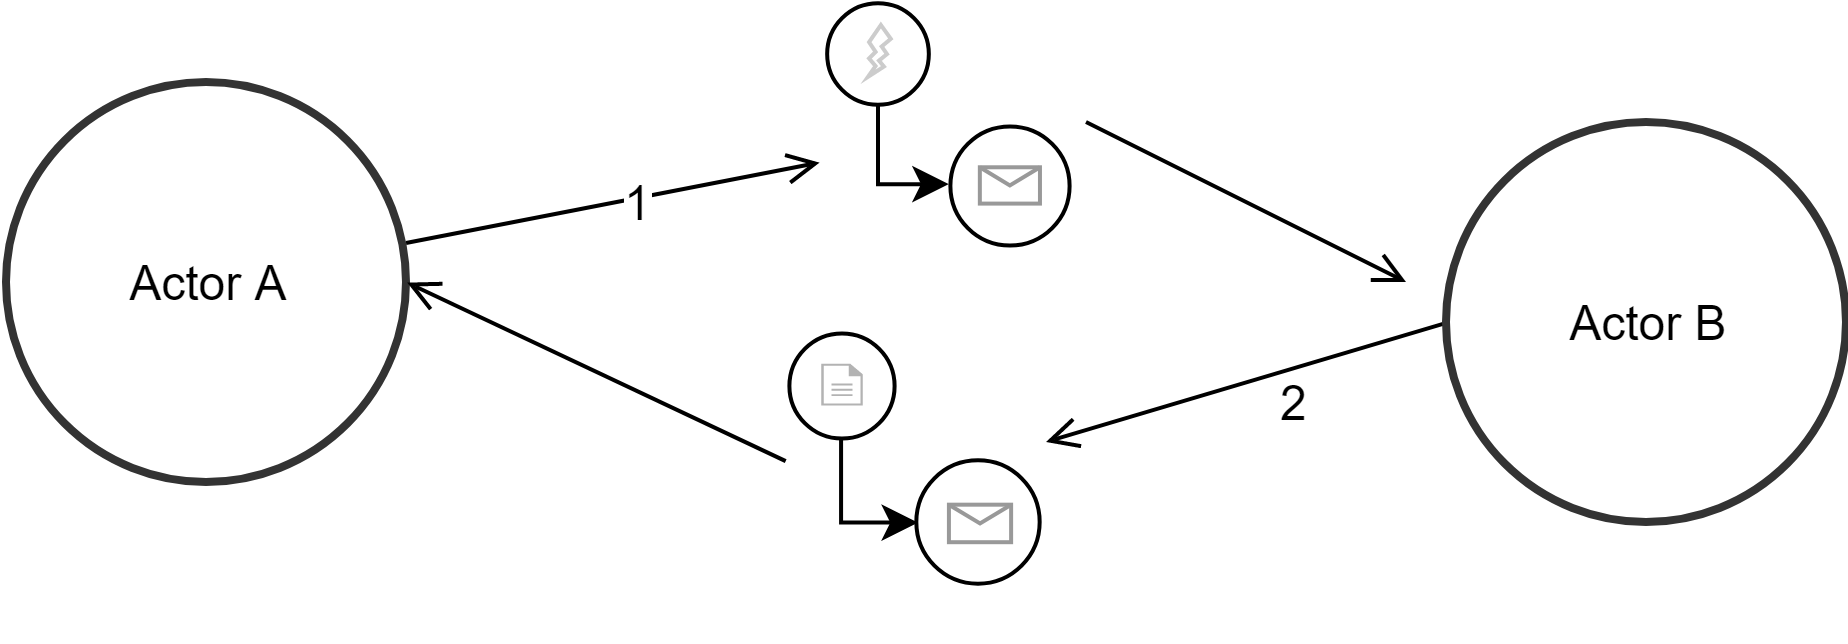
\includegraphics[width=\linewidth]{gfx/actor/patterns/requestReplay}
    \caption{Das \textit{Request-Replay} Pattern}
    \label{fig:actor:patterns:requestReplay}
\end{figure}

% todo correlation identifier erklären

\subsection{Return Adress}
Damit ein Actor eine Nachricht an einen anderen Actor senden kann, benötigt er wie in \ref{sec:actors:messages} erklärt, eine Adresse dessen. Diese kann auch in einer bereits empfangenen Nachricht enthalten sein. \\
In Abbildung \ref{fig:actor:patterns:returnAdress} ist zu sehen das ein Actor ein \textit{Command} and einen anderen Actor sendet, und in diesem \textit{Command} anweist die Antwort an einen seiner \textit{Childs zu senden}. \\
Diese so bekannt gegebene Adresse könnte auch für zukünftige Verarbeitungen von Nachrichten verwendet werden. In \cite{Vernon2015ReactiveAkka} wird beispielsweise ein Server/Client Prinzip zwischen Actors besprochen. Der Client-Actor bekommt dann zu beginn seines Lebenszyklus die Adresse eines Server-Actors übermittelt. Alle Informationen die der Client im weiteren verlauf erarbeitet, werden dann an den Server übermittelt.
\subsubsection{BILD RETURN ADRESS}\label{fig:actor:patterns:returnAdress}

\subsection{Processor}


\subsection{Routing}

\subsection{Aggregator}

\subsection{Grantierte Nachrichtenzustellung}
AtLeastOnceDelivery




